\documentclass[aspectratio=169]{beamer}
\usetheme{CambridgeUS}
\usecolortheme{default}

\useinnertheme[shadow=false]{tcolorbox}
\tcbthemeset{fuzzy halo=1mm with gray}

\title{Week 0: Course Orientation}
\subtitle{Stat 195: Midyear Bridge Program}
\author{Dominic Dayta}

\begin{document}

\begin{frame}
    \titlepage
\end{frame}

\begin{frame}{Session Overview}
    \tableofcontents
\end{frame}

\section{Course Introduction}
\section{Introduction to Statistics}

\begin{frame}{Methods of Statistics: The Origins}
    \textbf{What is Statistics?} \\
    Statistics is the original \textbf{information science}: pioneering statistical methods demonstrated early ideas in pattern recognition.

    \begin{columns}
        \begin{column}{0.5\textwidth}
        \small
            Under the new field of \textbf{biometrics}, Karl Pearson and Francis Galton attempted to explain natural selection by \textbf{collecting and summarizing} massive datasets involving the body measurements of different species.
        \end{column}
        \begin{column}{0.5\textwidth}
            \begin{center}
                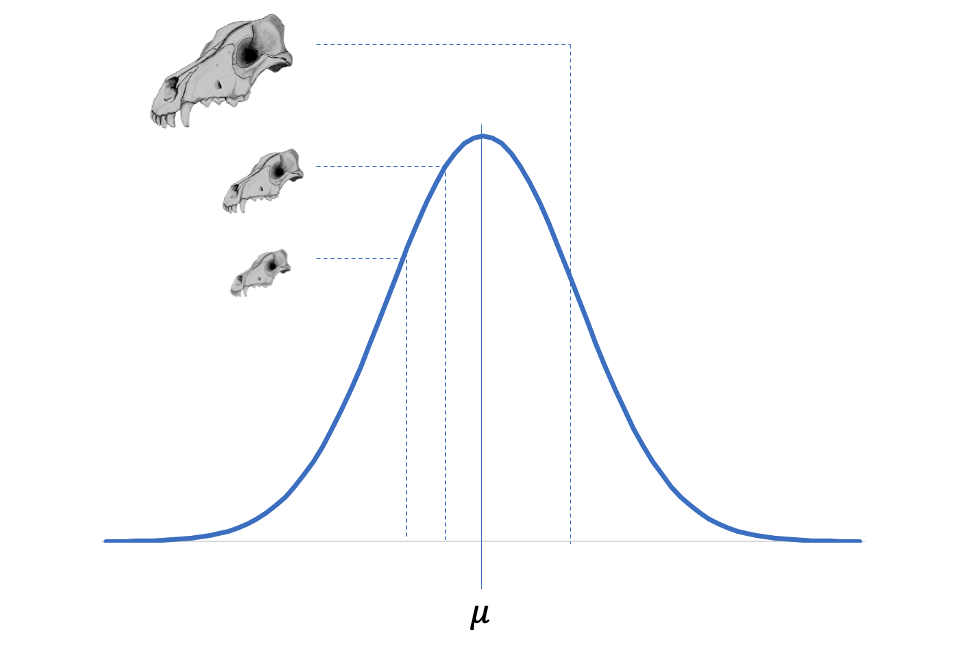
\includegraphics[width=0.9\textwidth]{images/biometrics.png}
            \end{center}
        \end{column}
    \end{columns}
\end{frame}

\begin{frame}{Methods of Statistics: Two Main Branches}
    \begin{itemize}
        \item \textbf{Descriptive statistics} involves the systematic collection, organization, summarization, and presentation of data. \emph{(Telling us what the data currently shows.)}
        \vspace{0.5cm}
        \item \textbf{Inferential statistics} enables us in drawing broader conclusions and making inferences about populations based on data obtained from samples. \emph{(Telling us what the data implies about the unknown.)}
    \end{itemize}
\end{frame}

\begin{frame}{Inferential Statistics: The Vocabulary}
    \begin{itemize}
        \item A \textbf{Population} refers to the entire set of subjects that are under study or consideration.
        \vspace{0.2cm}
        \item We are typically interested in a \textbf{parameter}: a summary measure that characterizes the population as a whole.
        \vspace{0.6cm}
        \item A \textbf{sample} refers to a smaller, representative subset of the population that is selected for observation and analysis.
        \vspace{0.2cm}
        \item When applied to the sample, the summary measure is called the \textbf{statistic}.
    \end{itemize}
\end{frame}

\begin{frame}{Exercise: Descriptive vs. Inferential}
    \small
    \textbf{Identify whether the following statements belong to Descriptive (DESC) or Inferential (INF) Statistics.}

    \vspace{0.3cm}
    \begin{enumerate}
        \item Analyzing server logs at Mind in a Device to determine the exact average response time of the primary API over the past week. \pause \hfill \textcolor{blue}{DESC} \pause
        
        \vspace{0.2cm}
        \item Using hardware performance data from a beta test of 500 users to predict the crash rate for a global software launch. \pause \hfill \textcolor{blue}{INF} \pause
        
        \vspace{0.2cm}
        \item A summary report detailing the exact number of bug tickets resolved in each module during the last development sprint. \pause \hfill \textcolor{blue}{DESC} \pause
        
        \vspace{0.2cm}
        \item Testing a random sample of 30 lithium-ion SFF batteries to estimate the mean lifespan of the entire production batch. \pause \hfill \textcolor{blue}{INF} \pause
        
        \vspace{0.2cm}
        \item An AI engineer uses cross-validation scores from a training set to estimate how well a model will generalize to unseen real-world data. \pause \hfill \textcolor{blue}{INF}
    \end{enumerate}
\end{frame}

\begin{frame}{Mathematical and Computational Statistics}
    \begin{itemize}
        \item \textbf{Classical statistics}, also known as \textbf{mathematical statistics} or simply \textbf{inferential statistics}, is rooted in mathematical theory and probability distributions.
        \vspace{0.3cm}
        \item Classical statistics emphasizes \textbf{theoretical foundations}, such as hypothesis testing, confidence intervals, and p-values, which are derived based on assumptions about data distributions and population parameters.
        \vspace{0.3cm}
        \item \textbf{Computational statistics} takes a more algorithmic and computational approach to statistical analysis. It leverages computational power and techniques to handle complex models, large datasets, and real-world scenarios that often violate classical assumptions.
    \end{itemize}
\end{frame}

\begin{frame}{Mathematical vs Classical Statistics}

\begin{center}
     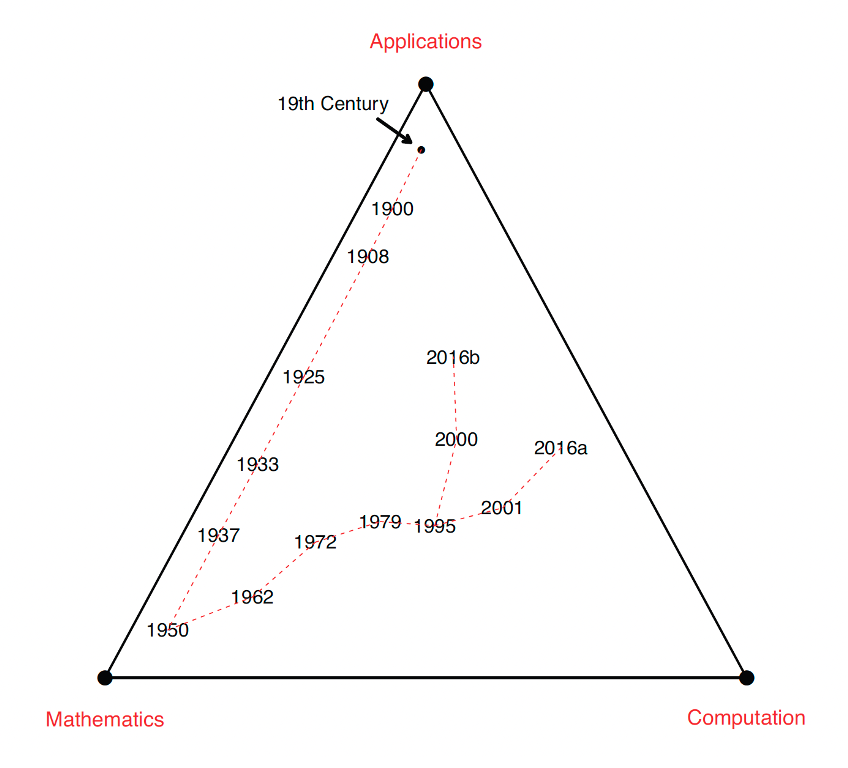
\includegraphics[width=0.4\textwidth]{images/method-triangle.png}
\end{center}

\end{frame}

\begin{frame}{A Very Slippery Typology}

\begin{center}
     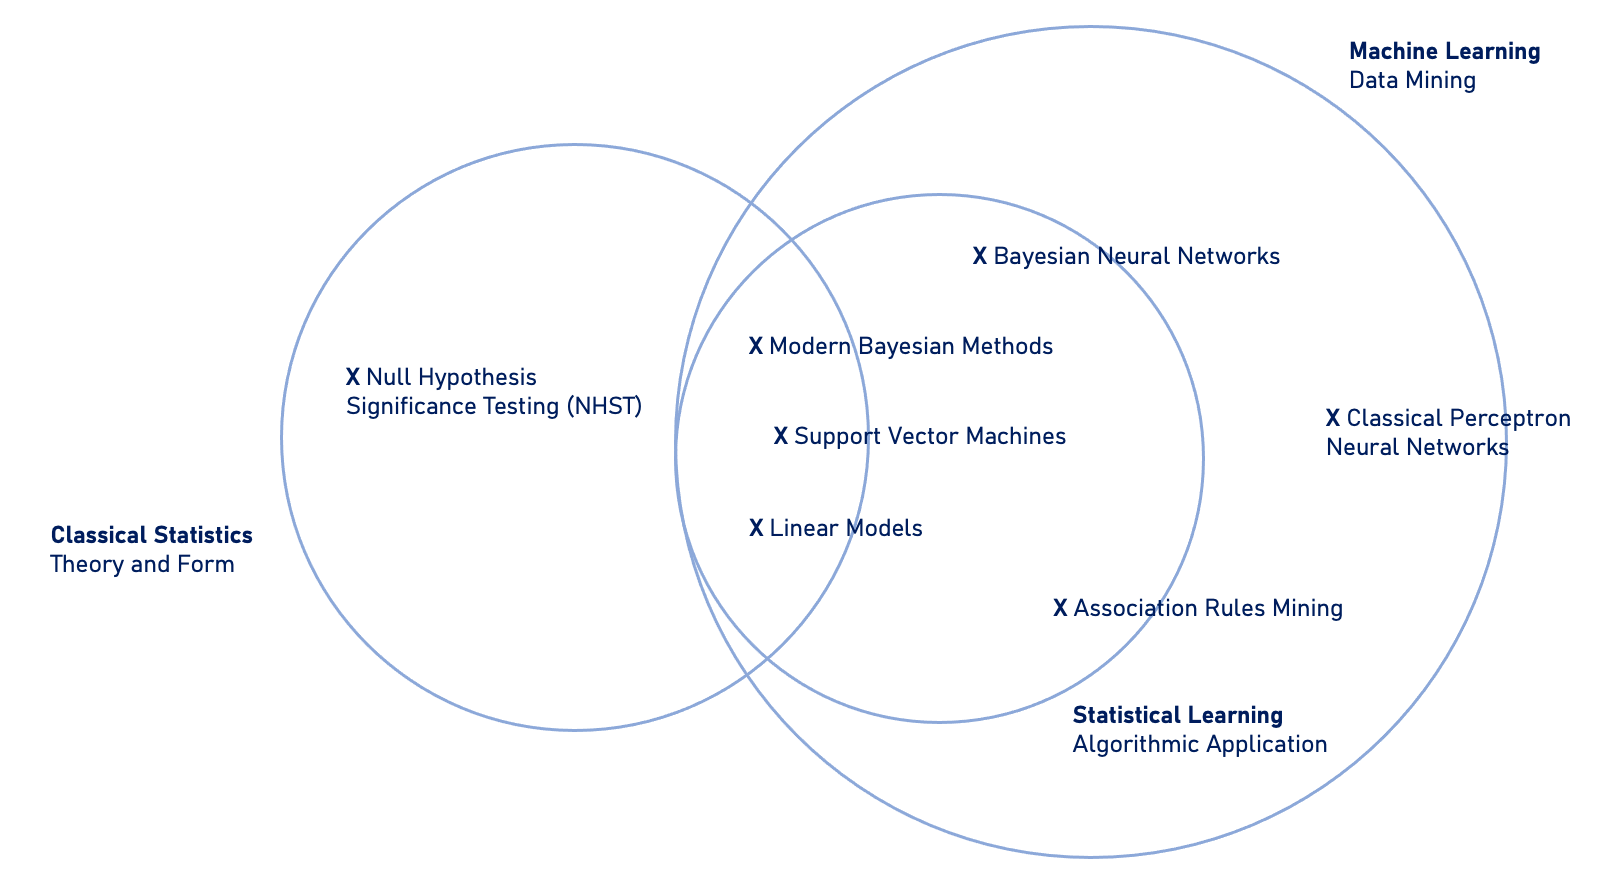
\includegraphics[width=0.8\textwidth]{images/typology.png}
\end{center}

\end{frame}

\begin{frame}{Exercise: Deconstructing Inference (Scenario 1)}
    \small
    A Lead Infrastructure Engineer at Mind in a Device wants to find out if there is a need to physically upgrade their edge servers. They wrote a diagnostic script to ping $1,000$ of the $3,000$ active edge servers in the regional network. The log results showed that $75\%$ of the $1,000$ tested servers experienced peak load latency above the acceptable threshold.
    
    \textbf{a) Identify the population and the sample.} \pause
    \begin{itemize}
        \item \textcolor{blue}{\textbf{Population:} All $3,000$ active edge servers in the regional network.}
        \item \textcolor{blue}{\textbf{Sample:} The $1,000$ edge servers pinged by the diagnostic script.}
    \end{itemize} \pause
    
    \textbf{b) Identify the variable of interest.} \pause
    \begin{itemize}
        \item \textcolor{blue}{\textbf{Variable:} Whether or not a specific server experienced high peak load latency. \textit{(Student Trap: The variable is NOT "the percentage." The variable is the binary Yes/No status recorded for each individual server.)}}
    \end{itemize} \pause
    
    \textbf{c) Identify the parameter and the statistic.} \pause
    \begin{itemize}
        \item \textcolor{blue}{\textbf{Parameter:} The true percentage of \emph{all} $3,000$ servers experiencing high latency.}
        \item \textcolor{blue}{\textbf{Statistic:} The $75\%$ observed in our specific sample.}
    \end{itemize}
\end{frame}

\begin{frame}{Exercise: Variables vs. Summary Measures (Scenario 2)}
    \small
    The core R\&D division is investigating the effectiveness of a new memory allocation algorithm in reducing the execution runtime of a massive neural network training pipeline. 
    
    \textbf{a) Identify the Population.} \pause
    \begin{itemize}
        \item \textcolor{blue}{\textbf{Population:} The theoretical set of all current and future training runs utilizing this specific memory allocation algorithm.}
    \end{itemize} \pause
    
    \vspace{0.4cm}
    \textbf{b) Identify the Variable(s) of interest.} \pause
    \begin{itemize}
        \item \textcolor{blue}{\textbf{Variable:} The execution runtime (in hours/minutes) of the pipeline before applying the algorithm, and the execution runtime after.}
        \vspace{0.2cm}
        \item \textcolor{blue}{\textbf{Student Trap:} "Average runtime" or "Difference in average runtime" is \textbf{INCORRECT} here. Averages are \emph{summary measures} (parameters/statistics). The \emph{variable} is simply "runtime", which is what you actually measure with a stopwatch on a single run.}
    \end{itemize}
\end{frame}

\begin{frame}{Exercise: Variables vs. Summary Measures (Scenario 3)}
    \small
    The cybersecurity team is interested in determining the percentage of legacy codebase repositories infected by a newly discovered zero-day vulnerability within the company's internal servers.
    
    \textbf{a) Identify the Population.} \pause
    \begin{itemize}
        \item \textcolor{blue}{\textbf{Population:} All legacy codebase repositories hosted on the company's internal servers.}
    \end{itemize} \pause
    
    \vspace{0.4cm}
    \textbf{b) Identify the Variable of interest.} \pause
    \begin{itemize}
        \item \textcolor{blue}{\textbf{Variable:} Whether or not a specific repository contains the zero-day vulnerability (Categorical: Infected / Not Infected).}
        \vspace{0.2cm}
        \item \textcolor{blue}{\textbf{Student Trap:} Do not say "The percentage of infected repositories." Percentage is a calculation done \emph{after} the data is collected. The variable is the raw data point collected from one single repository.}
    \end{itemize}
\end{frame}


\end{document}
